\documentclass[namedate,webpdf,contemporary,large]{TBench-template}
\usepackage[english]{babel}
\usepackage{graphicx}
\usepackage{amsmath}
\begin{document}
\journaltitle{BenchCouncil Transactions on Benchmarks, Standards and Evaluations}
\DOI{}
\appnotes{Research Article}
\firstpage{1}
\title[Label coverage bounds]{Label Coverage Bounds Pooled Macro F1 in Closed-Set Benchmarks}
\author[1,$\ast$]{Shah Zaib Sajid}
\authormark{Sajid}
\address[1]{\orgname{Independent Researcher}}
\corresp[$\ast$]{Correspondence: shahzaibjanjua25@gmail.com}
\abstract{A classifier's benchmark score depends on which test labels its output vocabulary permits. On the official NSL-KDD split, only 21 of 38 fine-grained test labels occur in training, capping pooled macro F1 at 0.55263 for training-restricted outputs. Across six prespecified pipelines, the forest leads full macro F1 while kNN leads covered-row scoring; two of fifteen pairwise rankings reverse. Rerouting only unavailable rows also changes the full-score winner without increasing true positives. CICIDS2017 day holdout gives the extreme case: every attack label is unavailable on its test day, so a forest's 0.06030 score lies below a ceiling of 0.06667, despite 0.85347 under shuffled cross-validation. We formalize the elementary coverage ceiling and a vocabulary oracle accounting for unavoidable false-positive destinations. The oracle is NP-hard for arbitrary vocabularies but fixed-parameter tractable in the number of destination labels by grouping repeated vocabularies. Released exact solvers implement this grouping and support explicit global output heads, positive-test-support scoring and inferred-label-union scoring. A fixed-cohort withholding grid examines destination-sensitive rankings; adjacent-batch gas sensing supplies a natural fractional case whose model-family rankings remain unchanged. A prospectively frozen literature screening pilot records eligibility and unresolved evidence without estimating field prevalence. The diagnostic separates legal-output restrictions from limited training support and model errors. It supplies an inspectable reporting step before fitting while leaving deployment validity and rare-class learnability to separate analyses.}
\keywords{Macro F1, vocabulary coverage, evaluation protocols, intrusion detection}
\maketitle
\section{Introduction}
A low benchmark score can describe two different failures: a model misclassifies a label it can output, or the evaluation asks it to name a label outside its output vocabulary. These failures have different remedies. Better features or fitting might address the first. They cannot address the second without changing the model's permitted decisions.

NSL-KDD illustrates the distinction without an artificial withholding rule. Its official test set contains 38 fine-grained labels, of which only 21 occur in training. For a classifier restricted to its training labels, even perfect classification of available rows cannot yield pooled macro F1 above 21/38, or 0.55263. Our seed-42 forest scores 0.25456. Mapping the same rows to the usual five categories restores complete coverage, but changes the recognition task. CICIDS2017 gives a more extreme example: all 14 attack labels are confined to individual capture days, so day holdout caps the 15-class pooled score at 1/15. The documented attack schedule is not a new discovery. Its implication for the attainable score is what we audit.

The recall constraint behind this ceiling is elementary. The additional question is where a closed-set classifier must send rows whose true label is unavailable. Those predictions create false positives somewhere. We define a vocabulary oracle that includes this loss, derive tractable cases and a polynomial-time sandwich, and establish hardness for unrestricted vocabularies. Grouping repeated vocabularies gives fixed-parameter tractability in the number of destination labels and is implemented in both exact solvers.

The empirical question is whether these constraints affect interpretation, rather than whether fitted scores obey a theorem. We examine label granularity, compare rankings on full and covered cohorts, and retain the legal-output distinction for global neural heads. A frozen sample of literature candidates documents what can be checked from accessible evidence. The intended contribution is a reporting diagnostic and its implementation, not a new detector or a universal measure of model quality.

\section{Related Work}
Security evaluations can become misleading when the sampling protocol answers a different question from the intended deployment setting \cite{sommer2010,arp2022}. Dataset surveys and CICIDS2017 audits document traffic-generation, feature and labeling limitations \cite{ring2019,engelen2021,lanvin2023}. We condition on the released labels and a declared partition; the present analysis neither repairs those datasets nor removes their other biases.

Macro F1 itself requires an explicit definition. Averaging class F1 differs from taking the harmonic mean of macro precision and recall \cite{opitzburst2019}. Pooling out-of-fold predictions also differs from averaging fold scores \cite{forman2010}. Work on classification metrics studies prevalence and prediction bias \cite{opitz2024,sokolova2009}, while confusion-matrix objectives can guide learning algorithms \cite{narasimhan2015}. Our optimization uses the true test labels to bound a fixed evaluation cohort; it is not a learning procedure.

Label shift concerns changed class priors under assumptions on conditional feature distributions \cite{lipton2018}. A missing legal output is a separate constraint: reweighting cannot create that output. Open-set recognition and selective prediction add unknown or reject decisions \cite{scheirer2013,geng2021,chow1970,geifman2019}. Generalized zero-shot learning permits unseen outputs through side information and evaluates seen and unseen recognition separately \cite{xian2017}. These settings explain why absence from training alone is insufficient to establish zero recall. Temporal and spatial discipline, as in TESSERACT \cite{pendlebury2019}, remains necessary even when every legal label is covered.

\section{A Score Limit from Legal Outputs}
Let \(f\) index folds, \(T_f\) their training labels, and \(V_f\ne\varnothing\) their legal output vocabularies. Assume a nonempty pooled test cohort. Every test row receives one label in \(V_f\). We allow \(V_f\) to contain labels absent from \(T_f\); training-restricted classifiers are the special case \(V_f=T_f\). Write \(n_{fk}\) for fold-level test support and define
\[
\begin{aligned}
S&=\{k:\textstyle\sum_f n_{fk}>0\},\quad n_k=\sum_f n_{fk},\\
m_k&=\sum_fn_{fk}\mathbf{1}\{k\in V_f\},\quad \rho_k=m_k/n_k\ (k\in S).
\end{aligned}
\]
The main metric pools confusion counts and averages class F1 over positive-test-support labels \(S\). This is an explicit scoring choice. It is not scikit-learn's default inferred union of true and predicted labels. Train-only or other output-only labels must remain in the vocabulary input even though they are excluded from this main average.

\paragraph{Proposition 1. Coverage ceiling.}
Every legal prediction vector satisfies
\[
F\le C=\frac{1}{|S|}\sum_{k\in S}\frac{2\rho_k}{1+\rho_k}.
\]
\emph{Proof.} A true positive needs a legal true label, hence \(TP_k\le m_k\) and recall is at most \(\rho_k\). Precision is at most one. Substitution in the increasing harmonic-mean expression for F1 proves the result. Equality needs every available row correct and no false positives entering a positive-\(m_k\) class.

Support-weighted F1 replaces \(1/|S|\) with \(n_k/\sum_jn_j\). Micro F1, with all true and predicted labels included, equals accuracy and is at most \(\sum_km_k/\sum_kn_k\). Balanced accuracy is at most \(|S|^{-1}\sum_k\rho_k\). These are deterministic cohort limits, not confidence intervals.

For leave-one-group-out using all remaining groups as training and \(V_f=T_f\), a label in one group has \(\rho_k=0\); a label in two or more groups has \(\rho_k=1\). Thus fractional pooled coverage requires another structure, such as a forward or restricted-window protocol. This explains both the severity and the simple form of the CICIDS2017 result.

\subsection{Legal outputs and limited training support}
A global head permitting every test label has \(C=1\), including when some labels have no training examples. This is the correct legal ceiling. It is not evidence that the missing classes can be learned. There is no distribution-free improvement based only on training counts: a feature can encode its correct global label, and a fixed classifier can decode it perfectly without any examples of that label. Conversely, the same counts can accompany uninformative features.

For sensitivity analysis, define \(V_f(\tau)=\{k:N^{\mathrm{train}}_{fk}\ge\tau\}\). Recomputing the bound describes how coverage changes with a declared support requirement. It is a hard ceiling only for a model that enforces this restricted vocabulary. Calling it a learnability ceiling for unrestricted networks would require additional assumptions about features, priors, side information and learning. The package therefore accepts legal vocabularies explicitly and uses training labels only as the default.

\section{The Vocabulary Oracle}
Correcting a wrong prediction on a row whose true label is legal cannot reduce macro F1: it adds a true positive to that class and removes a false positive from the old destination. After these repairs, let \(U_f=\sum_{k\notin V_f}n_{fk}\) be the unavailable rows and \(a_{fk}\) their destination counts. They satisfy \(a_{fk}\ge0\), \(a_{fk}=0\) outside \(V_f\), and \(\sum_ka_{fk}=U_f\). With \(a_k=\sum_fa_{fk}\), the maximum legal score is
\[
O=\max_a\frac{1}{|S|}\sum_{k\in S}\frac{2m_k}{n_k+m_k+a_k}.
\]
The oracle knows test truth and can choose destinations freely. It bounds a score; it does not estimate achievable deployment performance. The gap \(O-F\) is the remaining score shortfall, not a causal estimate of model quality.

\paragraph{Theorem 1. Vertex allocation.}
An optimum repairs all available rows and sends all unavailable rows in each fold to one legal destination. For \(m_k>0\), the second derivative of \(2m_k/(n_k+m_k+a)\) is \(4m_k/(n_k+m_k+a)^3>0\); a zero-\(m_k\) term is constant. The objective is convex on a product of allocation simplexes. A maximum has a vertex representative, and each such vertex assigns an integer number of rows to one destination per fold.

Let \(g_k(a)=2m_k/(n_k+m_k)-2m_k/(n_k+m_k+a)\) on \(S\), and zero outside \(S\). A fold can avoid any loss from \(C\) exactly when it permits a destination outside \(S\) or with \(m_k=0\). Consequently \(O=C\) exactly when every unavailable fold has such a destination. For a single unavailable fold,
\[
O=C-\min_{k\in V_f}g_k(U_f)/|S|.
\]
This also applies to any number of unavailable folds with one common vocabulary after summing their row counts. For a general input, set \(c_f=\min_{k\in V_f}g_k(U_f)/|S|\). Concavity, monotonicity and \(g_k(0)=0\) give
\[
\max(0,C-\sum_fc_f)\le O\le C-\max_fc_f.
\]
Sending each fold to its own minimum-loss destination proves the lower bound by subadditivity; any allocation incurs at least each individual minimum loss. These polynomial-time bounds remain available when exact search reaches its budget.

\subsection{Complexity and repeated vocabularies}
\paragraph{Theorem 2. General hardness.}
Computing the exact oracle for arbitrary vocabularies is NP-hard. Reduce from Set Cover with \(K\) candidate sets. Give each set a destination label and one coverable anchor row. For each element create \(L=2K+1\) rows of an unavailable label in a fold permitting exactly the sets containing that element. Assume each element belongs to a set. Theorem 1 assigns each element to one set. Occupied destinations form a cover. If their number is \(q\), the unaveraged loss is \(\sum_{a_k>0}a_k/(2+a_k)\), and
\[
q-1<qL/(L+2)\le\sum_{a_k>0}a_k/(2+a_k)<q.
\]
The intervals are disjoint, so the exact optimum identifies the minimum cover size. The construction is polynomial. This is a worst-case result, not a claim about difficulty on a named benchmark.

\paragraph{Theorem 3. Parameterization by destination labels.}
If no row is unavailable, \(O=C=1\). Otherwise, if the union of legal destinations in unavailable folds contains \(q\) labels, there is an exact algorithm using at most
\[
\prod_{j=1}^{q}j^{\binom{q}{j}}\le q^{2^q-1}
\]
candidate allocations and polynomial work per candidate. Group folds by identical vocabulary \(V\) and sum their unavailable counts. The Minkowski sum of their simplexes is the simplex with that summed mass. Convexity again gives an optimum placing the whole group at one destination. There are at most \(2^q-1\) nonempty vocabularies, proving the bound and fixed-parameter tractability in \(q\). The candidate bounds for \(q=2,3,4\) are 2, 24 and 20,736. The growth is rapid; this result does not promise efficient exact search for large \(q\).

Both enumeration and branch-and-bound implement grouping. Branch-and-bound uses the partial score before remaining false positives are charged as a completion upper bound, starts from a feasible greedy assignment and merges equivalent states. A node-budget exception certifies no optimum. Fixed uncovered-fold count instead gives an XP enumeration bound; it is a different parameterization. An independent pseudo-polynomial count-grid MILP and solver checks are in the supplement.

\subsection{Other scoring conventions}
If a scorer infers the union of true and predicted labels, let \(W\) be the activated outputs outside \(S\). Its denominator is \(|S|+|W|\), while those additional classes contribute zero. The coverage ceiling remains valid. Vertex allocation and vocabulary grouping still admit an optimum: fix the outside labels used by an optimum, maximize its convex numerator over those decisions, and take a vertex. Activating a subset of those outside labels can only improve the denominator.

If \(U_S\) bounds the oracle after restricting vocabularies to \(S\), use zero when this restriction is infeasible. With outside outputs available, a valid bound is \(\max\{U_S,C|S|/(|S|+1)\}\). Otherwise use \(U_S\). The software offers exact support and union objectives. A weighted average of fold scores instead has ceiling \(\sum_f\alpha_fC_f\) using each fold's scored inventory. For CICIDS2017 the equal-fold ceiling is 0.39000, distinct from pooled 0.06667.

Abstention scored as a miss without a false positive reaches \(C\): repair available rows and abstain on the rest. A scored unknown class changes both the target and the allowed decisions and needs a new audit. Neither convention permits exact recognition of an unavailable fine-grained label.

\section{Evaluation Design}
We use CICIDS2017 \cite{sharafaldin2018}, the official UNSW-NB15 partitions \cite{moustafa2015}, original-label NSL-KDD \cite{tavallaee2009}, and the UCI gas-sensor drift archive \cite{gasdata}. Counts, input hashes, membership manifests and confusion matrices accompany the code. All headline results use pooled positive-test-support macro F1 and source-training-label outputs. UNSW and NSL forests use 200 trees; CIC forests use 100 trees. Seeds 42--46 describe initialization variation on fixed cohorts, not independent networks or test sets.

CICIDS2017 compares five-fold stratified shuffled cross-validation with capture-day holdout. Numeric imputation uses training medians; web-label spelling variants are normalized. The local MachineLearningCVE CSVs contain no timestamps. A historical within-day row-order result is retained in the artifact but is not described as a verified temporal cutoff. All six archived forest configurations, including bootstrap weighting and that historical split, have separate fresh replication records agreeing with archived metrics to \(10^{-12}\).

NSL-KDD uses its named training and test files, one-hot nominal encoding and five forest seeds. UNSW uses training-fitted ordinal nominal encoding. Its controlled study withholds every pair of the nine attack labels, retains all original test rows and repeats 36 pairs over five seeds. For ranking analysis we separately save confusion matrices on available and unavailable rows. Full scores retain all ten test labels; covered-only scores retain the labels with positive support in that subset. Comparisons across different pairs consequently change the covered target and are descriptive condition comparisons.

The gas study fits batch \(t\) and tests batch \(t+1\), for nine adjacent-batch folds, a protocol used in drift research \cite{gasprotocol}. The 19 fits span forests, MLPs, histogram boosting, logistic regression, SVM, kNN and CORAL logistic regression \cite{coral2016}. CORAL uses unlabeled target features and is transductive. It retains source labels. Ranking statistics use fixed predictions; shared rows and overlapping training conditions preclude iid significance claims.

\section{Results}
\subsection{NSL-KDD: a natural partial-coverage split}
Of the 38 test labels, 17 are unavailable to a training-restricted classifier. The ceiling and support-scored oracle are both 0.55263. Two train-only labels supply destinations that cost nothing under positive-test-support scoring. Retaining them in the input matters: under inferred-union scoring the exact oracle is 0.54837. The seed-42 forest scores 0.25456, correctly classifying 16,287 of 18,794 available rows and none of 3,750 unavailable rows. Missing exact labels explain a substantial attainable-score restriction, although considerable error remains below the oracle.

The five-category mapping has ceiling one. This does not repair fine-grained recognition; it asks whether the system identifies a broader category. Reporting a high category score and a low fine-label score as interchangeable evidence would obscure this distinction.

\begin{table}[h]\centering
\caption{Natural NSL-KDD split: rankings change when unavailable rows are removed. Same fitted forests and test rows; covered scoring uses its positive-support inventory.}
\begin{tabular}{rrr}
Seed & Full macro F1 & Covered macro F1\\
42 & 0.25456 & 0.48702\\
43 & 0.23488 & 0.45491\\
44 & 0.23764 & 0.45548\\
45 & 0.23850 & 0.45566\\
46 & 0.23205 & 0.45612\\
\end{tabular}\end{table}
Spearman correlation across the five seeds is 0.40 and Kendall correlation is 0.40. Three of ten seed pairs reverse order. Seed 46 is second on covered rows but last on the full cohort; seed 42 leads both. This is an observed initialization-ranking inversion on a published natural split. It does not establish a reversal of published model-family conclusions, nor justify selecting a model using test labels. The differing false-positive destinations on unavailable rows help explain why full scoring need not preserve the covered-row order.


\paragraph{Prespecified pipeline comparison.}
We evaluated six declared pipelines on this natural split. The reference forest retains its original preprocessing. Five additional baselines use training-fitted numeric standardization and one-hot encoding; their parameters were fixed before fitting and no model was dropped after scoring. Forest, kNN and decision-tree full scores are close on this cohort, while their conditional scores differ more.
\begin{table}[h]\centering
\caption{NSL-KDD pipelines, seed 42 where applicable. Full and covered scores answer different recognition questions. Routed full F1 is a post-hoc oracle-assisted counterfactual on the original full cohort.}
\begin{tabular}{lrrr}
Pipeline & Full F1 & Covered F1 & Routed full F1\\
Random forest & 0.25456 & 0.48702 & 0.26914\\
Extra Trees & 0.22272 & 0.45041 & 0.24891\\
Decision tree & 0.25052 & 0.50858 & 0.28106\\
Gaussian NB & 0.17968 & 0.34711 & 0.19183\\
SGD logistic & 0.20806 & 0.40630 & 0.22453\\
kNN & 0.25160 & 0.53995 & 0.29839\\
\end{tabular}\end{table}
The forest leads full macro F1 (0.25456), whereas kNN leads covered-row scoring (0.53995). The forest falls to third on the covered subset (0.48702), below kNN and the decision tree. Two of fifteen pipeline pairs reverse order; Spearman correlation is 0.82857 and Kendall correlation is 0.73333. This changes the leading pipeline for the conditional recognition question on a natural split. The full metric remains valid for its declared exact-label task. These fixed-cohort outcomes do not establish ranking stability on independent networks or superiority of one estimator under identical preprocessing.

A post-hoc destination check keeps the original full cohort and metric. It reroutes only unavailable rows to spy, the alphabetically first legal train-only label, while preserving every covered-row prediction. The forest's full score becomes 0.26914 and kNN's 0.29839, reversing their original full-score order. Their true-positive counts remain exactly 16,287 and 15,869, respectively. Inferred-union scoring gives the same winner reversal. The routing uses true availability and a label with no test support; it diagnoses destination sensitivity and is not a deployable unknown-attack policy. This mechanism changes a model comparison without improved exact recognition.

\subsection{CICIDS2017: a day holdout changes the scoring task}
Every attack class appears on one day. Benign traffic remains available whenever tested, giving \(\rho_{\mathrm{BENIGN}}=1\); the 14 attack fractions are zero. Hence \(F=F_{\mathrm{BENIGN}}/15\) and \(C=O=0.06667\). The unweighted forest's score changes from 0.85347 in shuffled cross-validation to 0.06030 in day holdout. Under the latter protocol the attack F1 terms are fixed at zero, so their contribution cannot distinguish these training-restricted classifiers.

\begin{figure}[h]\centering
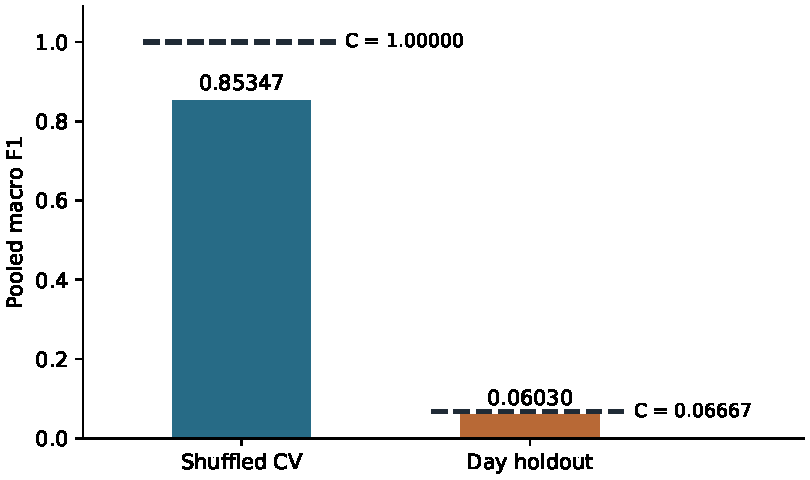
\includegraphics[width=0.95\columnwidth]{figures/cic_hero.pdf}
\caption{CICIDS2017 unweighted forest. Shuffled cross-validation has full label coverage; day holdout makes all fine-grained attack labels unavailable. The ceiling is a property of each protocol.}
\end{figure}

The day-held-out unweighted forest has benign recall 0.99858. Of the 557,646 unavailable attack rows, 475,727 are sent to benign and the remainder to other attack labels. Those other attack labels have zero covered support in the pooled score, so they provide free oracle destinations. This explains why the exact oracle equals the coverage ceiling here. The micro ceiling is 0.80300 because benign dominates the cohort. Merging web labels gives a 13-label ceiling of 0.07692; the declared eight-family mapping gives 0.25; binary attack detection has ceiling one. These are different evaluation targets.

\subsection{Fixed-cohort withholding and rankings}
The official UNSW-NB15 split has complete coverage. The unweighted forest's five-seed mean is 0.47144, with seed SD 0.00094. Training-label availability cannot explain that shortfall. Withholding two labels creates \(C=0.8\), but its oracle depends on their support and legal destinations. For Analysis plus Backdoor at seed 42, \(O=0.79833\) and \(F=0.47067\).

Across all 180 pair/seed conditions, full and covered-row scores have Spearman correlation 0.84862 and Kendall correlation 0.68007; 2,577 of 16,110 pairwise comparisons reverse order. Across the 36 pair means, Spearman correlation is 0.85174, with 97 of 630 orders reversed. Within a fixed withheld pair, 49 of 360 seed-pair comparisons reverse; 22 of 36 withholding conditions have at least one reversal. The across-pair summaries combine different covered label sets and are descriptive comparisons of conditions. Within-pair summaries hold that target fixed. All 180 full scores reproduce the earlier grid to absolute tolerance $10^{-12}$; the fresh matrices additionally make covered scoring reconstructible. No iid correlation interval or significance claim is attached to these dependent fits.

An oracle-assisted intervention changes only the destination predictions of unavailable rows, routing them to the training-majority label. Among the 65 newly fitted conditions with this routing record, full macro F1 increases by as much as 0.08262 without one additional true positive. It uses true availability and is a diagnostic counterfactual, not an implementable unknown-attack detector. A fixed confidence threshold of 0.5 has mixed effects. These results show that full macro F1 can reward destination changes separately from improved exact recognition.

\subsection{Natural fractional coverage and model families}
In adjacent-batch gas sensing, toluene is unavailable when batch 6 is tested. That fold contains 467 of its 1,759 pooled test rows, giving \(\rho=1292/1759\). The other five classes have full coverage. Global label presence misses this fold-level restriction: all six labels occur somewhere in training.

\begin{table}[h]\centering
\caption{Different natural protocols retain their own targets. \(O-F\) is a score shortfall, not an estimate of model quality.}
\begin{tabular}{lrrr}
Case & C & O & F\\
NSL original, forest & 0.55263 & 0.55263 & 0.25456\\
CIC day, forest & 0.06667 & 0.06667 & 0.06030\\
Gas, forest & 0.97449 & 0.96222 & 0.57034\\
Gas, logistic & 0.97449 & 0.96222 & 0.61946\\
\end{tabular}\end{table}
The gas oracle tightens the coverage ceiling by 0.01227. Its restriction from one explains 8.8\% of the forest's shortfall and 9.9\% of logistic regression's. It explains zero toluene hits in batch 6 but little of the pooled shortfall. Across all 19 gas fits, full and covered-only rankings agree exactly: Spearman and Kendall correlations are one, with 161 concordant comparisons and ten ties. The model-family contrast therefore provides no natural family-ranking reversal. CORAL logistic scores 0.63760 while retaining the same legal ceiling.

\subsection{Algorithm checks and literature screening}
Exhaustive row-level enumeration on 80 small seeded inputs agrees with both solvers under support and union scoring. Another 100 cases with explicitly supplied legal heads, including labels absent from training, agree with exhaustive predictions. A repeated-vocabulary check reduces 300 unavailable folds from \(2^{100}\) candidate assignments to two. These checks validate implementation and edge cases; fitted scores lying below a theorem are not independent evidence of significance. Varied synthetic shapes still reach exact-search budgets, as documented in the supplement.

A local protocol was committed before collecting six Crossref searches, each retaining the first 100 relevance-ranked records dated 2017--2026. Title filtering and DOI deduplication yielded 385 candidates. NumPy seed 20261108 selected 50 without replacement. The public frame, source metadata, sample, checksum and coding sheet are retained. This is a prospective local freeze rather than external preregistration.

Screening confirmed three eligible evaluations, excluded fourteen records and left thirty-three eligibility decisions unresolved. Temporal neuron coding and split learning were frequent reasons not to infer evaluation timing from a title. Of the three confirmed cases, one binary source-to-target evaluation permits both labels and therefore has legal ceiling one; its exact F1 averaging remains unresolved. The other two lack verified vocabulary/support/scoring information. No complete incompatible-score comparison is established. The result is a candidate-screening pilot, not a survey of fifty confirmed temporal IDS papers or a field prevalence estimate. Accessible abstract evidence can establish eligibility without establishing a score convention; missing evidence is retained as missing. The separate targeted source checks and DOI verification are in the supplement and artifact.

\section{Using the Diagnostic}
Choose the evaluation target before optimizing a split. Stratified shuffled cross-validation can measure interpolation over a shared inventory but does not establish future-day generalization. A chronological or capture-group holdout addresses a different deployment question and should retain the availability audit. Leave-one-attack-class-out should specify a binary alarm or a scored unknown target when the aim is unfamiliar-attack detection. Exact identification of a withheld fine-grained label cannot measure that capability for a training-restricted output head.

The reporting sequence is short: preserve fold membership; state the legal vocabulary and per-class support; declare pooling and the scored labels; compute \(C\), then \(O\) or its sandwich if destination loss matters; report full and covered-row scores with their respective inventories. State whether labels come from training or a global head. A ratio \(F/O\), when \(O>0\), describes attainment on that cohort only and should accompany the absolute score. It cannot make different targets or populations comparable.

The package exposes fold-array and count-based interfaces, accepts an explicit legal vocabulary per fold, and supplies a CLI for count files. Reproduction commands and a table-to-file map accompany the release. Counts, software, manifests and checksums are public artifacts; raw traffic redistribution remains subject to dataset terms.

\section{Limitations and Conclusion}
The simple ceiling is a scoring corollary of legal-output constraints. It does not measure feature separability, rare-class learnability, calibration or deployment utility. The exact oracle adds unavoidable false-positive loss and admits a vocabulary-parameterized algorithm, but this correction is small in the natural examples considered. The NSL-KDD pipeline winner and seed-ranking reversals demonstrate score sensitivity on our fitted baselines; they are not a reanalysis that overturns a published model comparison. Shared-cohort repetitions describe fixed experiments rather than population uncertainty.

The literature screening has a bounded search frame and unresolved sources. It cannot support a field-wide prevalence claim. No verified incompatible published score is established. Timestamped CIC files and corrected label releases are absent locally, and a file-verified CICDDoS2019 study is not supplied. A permanent DOI, an externally hosted anonymous artifact and independent reproduction also remain pending.

The main practical conclusion is narrower than a new detector claim: a benchmark score should be interpreted against the decisions its protocol permits. NSL-KDD shows natural partial coverage; CICIDS2017 shows an extreme day-holdout restriction; the gas comparison shows that coverage can explain little. Reporting these outcomes, including the null ranking result, makes the diagnostic useful without overstating its reach.

\section*{Data availability}
Dataset sources are cited above. The accompanying code release contains aggregate results, split manifests, hashes, source coding and commands mapped to the manuscript. Original data terms continue to apply.
\section*{Declarations}
This research received no funding. The author declares no financial or non-financial competing interests.
\section*{Use of generative AI}
Generative AI assisted code development, mathematical exposition, literature screening, analysis planning and manuscript editing. Numerical results were computed with the released scripts. The author retains responsibility for the submitted work.
\bibliographystyle{TBench}
\bibliography{references}
\end{document}
